\subsection{Communications (COMM)}
Due to the fact that the main objective of the mission is to provide internet
communications along the globe, this subsystem is considered critical for the
mission success. The communications subsystem (COMM) will be the one in charge
of providing effective transmission and reception of the radio signals between the
satellite and both the ground stations and other satellites, within \MissionName
constellation or third part satellites.

\subsubsection{Design process}
In order to design the communications subsystem, we have to identify which are
the communication needs of our satellites. That needs can be categorized in two types:

\begin{itemize}
	\item \textbf{Ground communications}. That are communications between the
	satellite itself with ground systems, both fixed ground stations (GS) and
	smaller, portable, IoT devices.
	\item \textbf{Inter-satellite communications}. Which are communication
	with other satellites in orbit, within our constellation or not.
\end{itemize}

This two needs sets a first requirement for the communications subsystem:
the antenna system shall be separated in two independent antennas, one for the
ground communications (in the following, called Earth-antenna) and another one for
the inter-satellite communications (called space-antenna). This approach as also the
advantage of some kind of redundancy; in case of failure of the Earth-antenna, the
satellite could still be operative as a inter-satellite link.

The two sets of antennas may have different base frequencies. The Earth-antenna
frequency is restricted by the Earth-atmosphere blocking frequencies shown in
figure \ref{fig:frequency_atmosphere_opacity}, so in the practice they are limited
to the radio frequency range from

\begin{figure}[h]
	\centering
	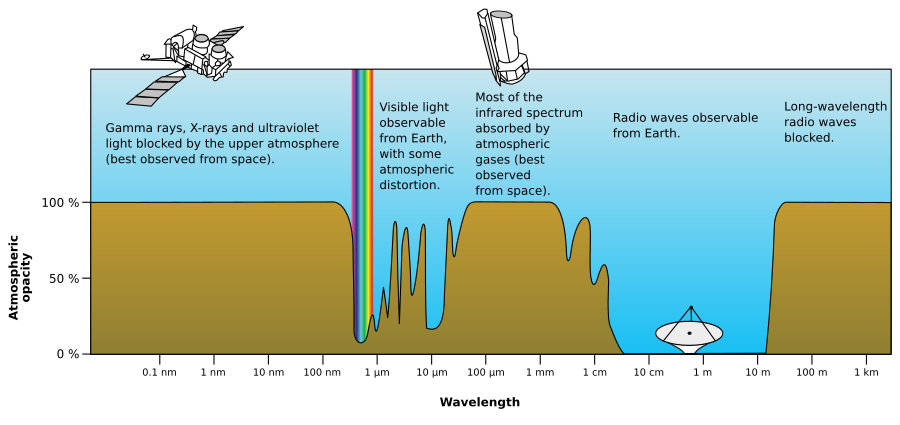
\includegraphics[width=\textwidth]{img/earth_freq.png}
	\caption{Atmospheric electromagnetic radiation opacity}
	\label{fig:frequency_atmosphere_opacity}
\end{figure}
